\documentclass[times, 10pt]{thesisMDH}
\usepackage[ddmmyyyy]{datetime}
\usepackage[pdfborder={0 0 0},colorlinks=true,urlcolor=blue,citecolor=red,bookmarks=false]{hyperref}
\usepackage{float}
\usepackage{makecell}
% \usepackage{indentfirst}
\setlength\parindent{0pt}

\university{University of Science and Technology of Hanoi}
\department{Information and Communication Technology}

\subject{Distributed System}
\thesisTitle{Practical Work 3:\\MPI File transfer}

\authorOne{Nguyen Phuong Thao}{BI9-212}
\authorTwo{Doan Tuyet Mai}{BI9-162}
\authorThree{Trinh Thao Phuong}{BI9-191}
\authorFour{Phung Kim Son}{BI9-202}
\authorFive{Pham Minh Long}{BI9-146}

\theDate{Hanoi, Feb 2021} 

\begin{document}
\titlePage

\newpage

\mainmatter

\section{Why you chose your specific MPI implementation}
In this labwork, we choose OpenMPI as the MPI implementation because it is easy to use. Also, OpenMPI is a high-quality implementation of MPI standard, with a large number of supports. The OpenMPI process manager seems to be very good and doesn’t have any noticeable weakness, that is really convenient for us to execute the MPI program.
\section{MPI service design}
\begin{figure}[H]
    \centering
    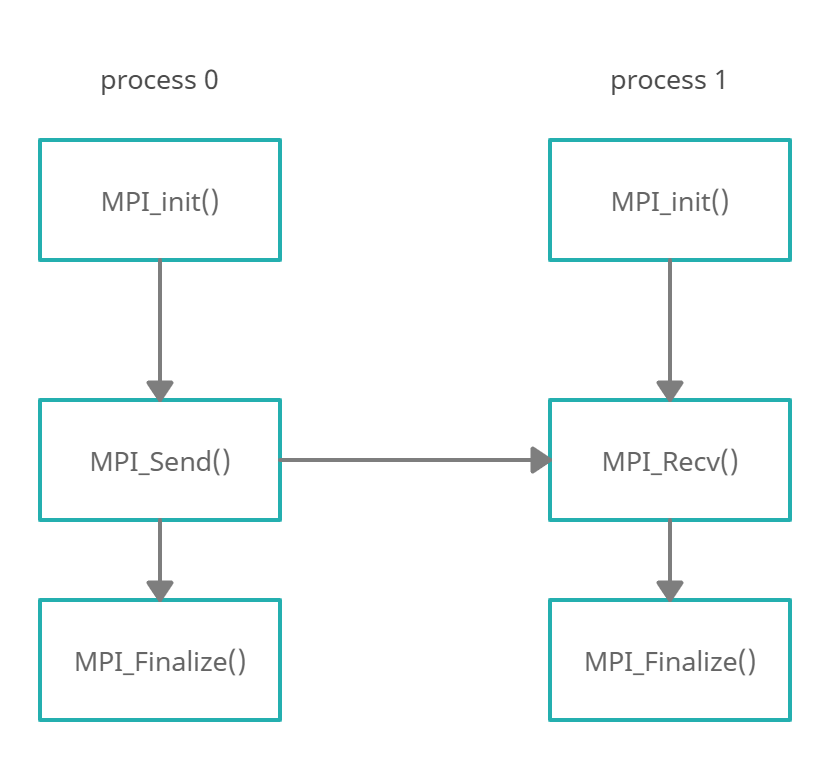
\includegraphics[width=0.7\linewidth]{images/3-1.png}
    \caption{MPI service design}
    \label{fig:my_label}
\end{figure}
First, we initialize MPI method on each process. On process 0, we execute the MPIsend() to send the text value in text file over the network. After that, the process 1 receive the content with the same rank and tag. When 2 processes finishing the tasks, the MPI will be destroyed by Finalize function.
\section{System organization}
\begin{figure}[H]
    \centering
    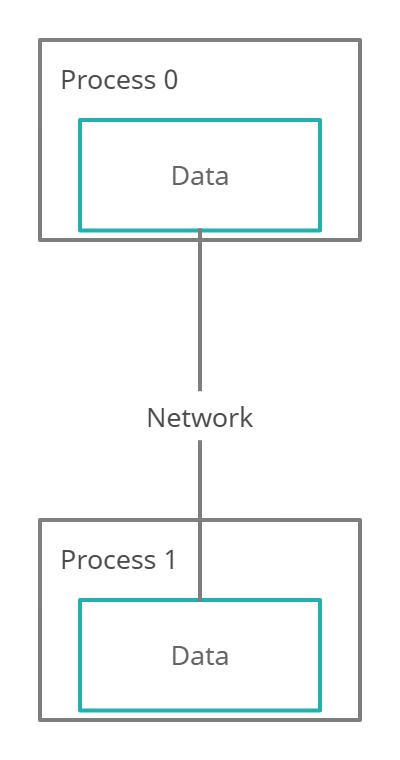
\includegraphics[width = 0.3\linewidth]{images/3-2.png}
    \caption{System organization}
\end{figure}

\section{File transfer implementation}
File content transfer code was mainly implemented in \texttt{mpi\_send\_file\_content.c} file. The header file \texttt{transfer.h} must be included.
First, the file reading function was implemented as following. The function was set to read the content of \texttt{test.txt} file
\begin{lstlisting}
 FILE *fptr;
    if ((fptr = fopen("test.txt", "r")) == NULL) {
        printf("Error! opening file");
        // Program exits if file pointer returns NULL.
        exit(1);
    }

    // reads text until newline is encountered
    fscanf(fptr, "%[^\n]", message);
    //printf("Data from the file:\n%s\n", );
    fclose(fptr);
\end{lstlisting}
Then, here is the initialization of the MPI program. The message length was set to at most 1000 characters.
\begin{lstlisting}
    int process_Rank, size_Of_Cluster, len;
    char message[1000];
    char name[MPI_MAX_PROCESSOR_NAME];

    MPI_Init(&argc, &argv);
    MPI_Comm_size(MPI_COMM_WORLD, &size_Of_Cluster);
    MPI_Comm_rank(MPI_COMM_WORLD, &process_Rank);
    MPI_Get_processor_name(name, &len);
    ....
    MPI_Finalize();
\end{lstlisting}
Message passing in MPI is handled by the corresponding functions and their arguments:
\begin{lstlisting}
    MPI_Send(&message, strlen(message), MPI_CHAR, 1, 1, MPI_COMM_WORLD);
    MPI_Recv(&message, strlen(message), MPI_CHAR, 0, 1, MPI_COMM_WORLD, MPI_STATUS_IGNORE);
\end{lstlisting}
In this case, we tried to send the content of the file from one processor to another processor. Then, here is the implementation of the sending part from the processor 0
\begin{lstlisting}
    if(process_Rank == 0){
    	//printf("Enter the message to sent: \n");
    	//scanf("%s",message);
        MPI_Send(&message, strlen(message), MPI_CHAR, 1, 1, MPI_COMM_WORLD);
        printf("Content of file test.txt sent from processor %s: %s\n", name, message);
    }
\end{lstlisting}
And here is the implementation of the receiving part from the processor 0
\begin{lstlisting}
    else if(process_Rank == 1){
        MPI_Recv(&message, strlen(message), MPI_CHAR, 0, 1, MPI_COMM_WORLD, MPI_STATUS_IGNORE);
        printf("Content of file test.txt received from processor %s: %s\n", name, message);
    }
\end{lstlisting}

\section{Contribution}
\begin{center}
    \begin{tabular}{|l|l|l|}
        \hline
        \textbf{Student} & \textbf{Student ID} & \textbf{Contribution}\\
        \hline
        Pham Minh Long & BI9-146 & System organization \\
        \hline
        Phung Kim Son & BI9-202 & File transfer implementation\\
        \hline
        Trinh Thao Phuong & BI9-191 & Draw figures\\
        \hline
        Doan Tuyet Mai & BI9-162 & MPI service design \\
        \hline
        Nguyen Phuong Thao & BI9-212 & Brief explanation\\
        \hline
    \end{tabular}
\end{center}

\end{document}
